\documentclass{article}

\usepackage[polish]{babel}
\usepackage[utf8]{inputenc}
\usepackage[T1]{fontenc}
\usepackage{enumitem}
\usepackage[onelanguage]{algorithm2e}
\SetKwInput{KwData}{Dane}
\SetKwInput{KwResult}{Wynik}
\SetKwRepeat{Do}{do}{while}
\usepackage{amsmath}
\usepackage{booktabs}
\usepackage{graphicx}
\usepackage{geometry}
\usepackage{multicol}
\geometry{
a4paper,
total={170mm,257mm},
left=15mm,
right=15mm,
top=30mm,
bottom=30mm
}
\title{Obliczenia Naukowe\\Lista 4\\Laboratoria}
\date{7 grudnia 2017}
\author{Piotr Szyma}


\begin{document}
    \pagenumbering{gobble}
    \maketitle
    \newpage
    \pagenumbering{arabic}
    \section{Zadanie 1}
\subsection{Opis problemu}
Napisać funkcję obliczającą ilorazy różnicowe zgodnie ze specyfikacją podaną w treści zadania bez użycia tablicy dwuwymiarowej (macierzy). \\ $ \texttt{function ilorazyRoznicowe (x::Vector{Float64}, f::Vector{Float64})} $ \\
\subsection{Analiza}
\subsection{Implementacja}
Moja implementacja algorytmu w języku Julia znajduje się w module $ \texttt{MyModule} $ znajdującym się w pliku załączonym do tego sprawozdania. 
    \newpage    
    
\section{Zadanie 2}
\subsection{Opis problemu}
Narysować wykres funkcji $ f(x) = e^x \ln (1 + e^{-x}) $ w co najmniej dwóch dowolnych programach do wizualizacji. Następnie policzyć granicę funkcji $ \lim_{x \to \infty} f(x) $. Porównać
wykres funkcji z policzoną granicą. Wyjaśnić zjawisko.
\subsection{Rozwiązanie}
Oto granica funkcji $ f(x) $:
$$ \lim_{x \to \infty} e^x \ln (1 + e^{-x}) = 1$$
\subsection{Wynik}
Wykresy wygenerowane za pomocą dwóch programów do wizualzacji załączone są na Rysunkach 1 i 2. Kody źródłowe programów dołączyłem do sprawozdania w osobnych plikach. \\\\
Jak widać na wykresach, w pewnym momencie funkcja zaczyna przyjmować nieoczekiwane - błędne - wartości. Głównym czynnikiem wpływającym na takie zachowanie jest operacja mnożenia bardzo dużej liczby $ e^x $ przez bardzo małą liczbę $ \ln(1 + e ^{-x}) $, bo $ \lim_{x \to \infty} \ln (1 + e^{-x}) = 0$.
\begin{figure}[!htbp]
  \centering  
  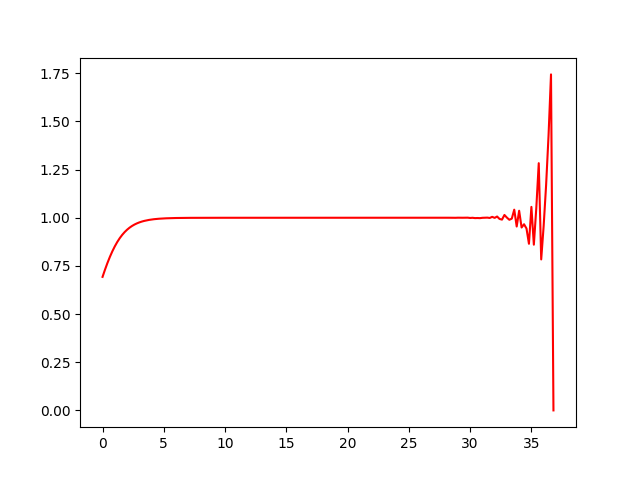
\includegraphics[totalheight=7cm]{../source/task-2/matplotlib.png}
  \caption{Wykres wygenerowany za pomocą biblioteki matplotlib w języku Python}
  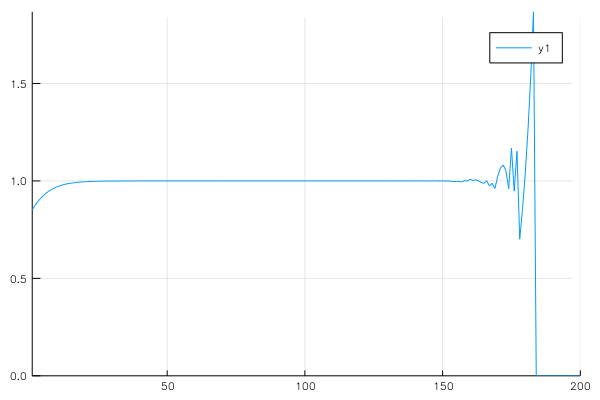
\includegraphics[totalheight=6cm]{../source/task-2/juliaplot.png}
  \caption{Wykres wygenerowany za pomocą biblioteki Plot w języku Julia}
\end{figure}

    \newpage
    \section{Zadanie 3}
\subsection{Opis problemu}
Zadanie polegało na zaimplementowaniu algorytmu rozwiązującego równanie $ f(x) = 0 $ $\textsc{metodą siecznych} $.
\subsection{Pseudokod}
\begin{algorithm}[H]
  \KwData{$f, a, b, M, \delta, \epsilon$}
  \KwResult{$x, f(x), i, err$}
  $f_a \leftarrow f(a);$ $f_b \leftarrow f(b)$\\
  \Do{$ k < M $}{
    $ k \leftarrow k + 1 $ \\
    \If{$ |f_a| > |f_b| $}{
      $a \leftrightarrow b$; $f(a) \leftrightarrow f(b)$ 
    }
    $ s \leftarrow \frac{b - a}{f_b - f_a}$ \\
    $ b \leftarrow a$; $ f_b \leftarrow f_a$  \\ 
    $ a \leftarrow a - f_a * s $  \\ 

    \If{$ |b - a| < \delta \lor |f_a| < \epsilon $}{
      return $ (a, f_a, k, 0) $;
    }
  }
  return $ (a, f_a, M, 1) $;  
\end{algorithm}
\subsection{Implementacja}
Moja implementacja algorytmu w języku Julia znajduje się w module $ \texttt{MyModule} $ znajdującym się w pliku załączonym do tego sprawozdania.
    \newpage
    \section{Zadanie 4}
\subsection{Opis problemu}
,,Złośliwy wielomian'' Wilkinsona. Zainstalować pakiet $ \mathtt{Polynomials} $.
\begin{enumerate}[label=(\alph*)]
  \item Użyć funkcji $ \mathtt{roots} $ z pakietu $ \mathtt{Polynomials} $ do obliczenia 20 zer wielomianu P zadanego w treści zadania. Sprawdzić obliczone pierwiastki $ z_k, 1 \leq k \leq 20 $, obliczając $|P(z_k)|$, $|p(z_k)|$ i $|z_k - k|$. Wyjaśnić rozbieżność. \\
  Zapoznać się z funkcjami $ \mathtt{Poly},\; \mathtt{poly},\; \mathtt{polyval}$ z pakietu $ \mathtt{Polynomials} $.
  \item Powtórzyć eksperyment Wilkinsona, tj. zmienić współczynnik $-210$ na $ -210-2^{-23}$. Wyjaśnić zjawisko.
\end{enumerate}
\subsection{Rozwiązanie}
Funkcja $ \mathtt{Poly(x)} $ generuje wielomian w zależności od współczynników podanych jako parametr.
Funkcja $ \mathtt{poly(x)} $ tworzy wielomian na podstawie pierwiastków wielomianu, natomiast funkcja $ \mathtt{polyval(p, x)} $ pozwala na wyliczenie wartości wielomianu $ \mathtt{p} $ dla zadanego argumentu $ \mathtt{x} $. Napisałem program z użyciem wyżej wymienionych funkcji z biblioteki $ \mathtt{Polynomials} $. Kody źródłowe dołaczyłem do sprawozdania. 

\subsection{Wynik}
Wyniki poszczególnych części zadań zamieściłem w tabelach poniżej - zatytułowanych odpowiednio (a) i (b). \\\\
Rozwiązując podpunkt (a) zadania zaobserwowałem pewne rozbieżności w wynikach. 
Porównując wartości $ P(z_k) $ oraz $ p(z_k) $ zauważyłem, że wyniki różnią się od siebie. 
Wyliczone za pomocą funkcji $ \mathtt{roots(P(x))} $ pierwiastki wielomianu $ P $ różnią się od jego rzeczywistych pierwiastków. Wnioskiem z poczynionych obserwacji jest fakt, że operacje wyznaczania wielomianu na podstawie współczynników czy tworzenia go z pierwiastków, są obarczone pewnym zaburzeniem, wynikającym z precyzji arytmetyki użytej do wykonania obliczeń. \\\\
Podpunkt (b) dotyczył złośliwego wielomianu Wilkinsona - zaburzania wielomianów tak, aby wykonywane na nich operacje numeryczne generowały duże rozbieżności od rzeczywistych wyników. Mała zmiana jednego ze współczynników sprawiła, że wyniki w podpunkcie (b) znacznie różniły się od punktu (a). Ta mała zmiana, przez którą wartość jednego z czynników wymagała dużej dokładności (aproksymowanej przez skończoną arytmetykę) wygenerowała duży błąd - przy każdej operacji korzystającej z tej liczby. Funkcja $ \mathtt{roots(P'(x))} $ wywołana na wielomianie z drugiego przykładu, zwróciła pierwiastki zespolone.
\newpage
\begin{center}
  \subsubsection*{Float64}
$$
\begin{array}{c|c|c|c|c}
algorytm & przed & \sigma & po & \sigma\\
\hline
1 & 1.0251881368e-10 & -1.1184955314e+01 & -4.2963427399e-03 & -4.2682954616e+08 \\
2 & -1.5643308870e-10 & -1.4541186645e+01 & -4.2963429987e-03 & -4.2682957187e+08 \\
3 & 0.0000000000e+00 & -1.0000000000e+00 & -4.2963428423e-03 & -4.2682955633e+08 \\
4 & 0.0000000000e+00 & -1.0000000000e+00 & -4.2963428423e-03 & -4.2682955633e+08 \\
\end{array}
$$
\subsubsection*{Float32}
$$
\begin{array}{c|c|c|c|c}
algorytm & przed & \sigma & po & \sigma\\
\hline
1 & -4.9994429946e-01 & -4.9668057661e+10 & -4.9994429946e-01 & -4.9668057661e+10 \\
2 & -4.5434570313e-01 & -4.5137965580e+10 & -4.5434570313e-01 & -4.5137965580e+10 \\
3 & -5.0000000000e-01 & -4.9673591353e+10 & -5.0000000000e-01 & -4.9673591353e+10 \\
4 & -5.0000000000e-01 & -4.9673591353e+10 & -5.0000000000e-01 & -4.9673591353e+10 \\
\end{array}
$$

\end{center}
    \newpage
    \section{Zadanie 5}
\subsection{Opis problemu}
Zadanie polegało na wygenerowaniu wykresów wielomianów interpolowanych z poniższych funkcji za pomocą wcześniej zaimplementowanych metod.
\begin{enumerate}
  \item $f(x) = e^x, [0, 1], n = 5, 10, 15$
  \item $g(x) = x^2 \sin(x), [-1, 1], n = 5, 10, 15$
\end{enumerate} 
\subsection{Rozwiązanie}
Na poniższych rysunkach przedstawiłem wykresy dla funkcji $f(x)$ oraz $g(x)$ dla poszczególych $n = 5, 10, 15$ 
\begin{figure*}
  \begin{multicols}{2}
        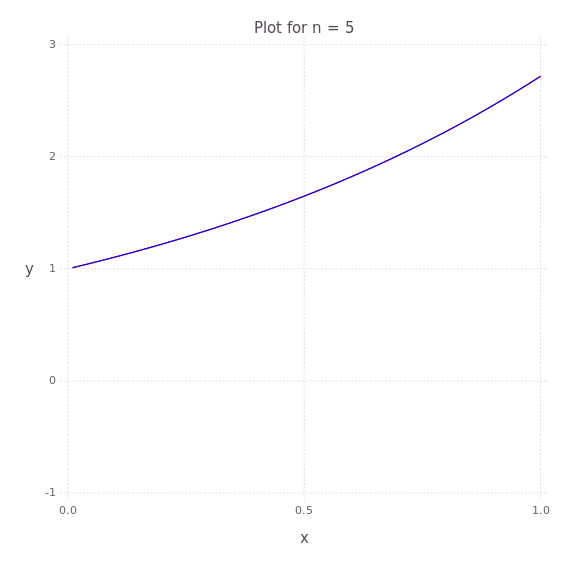
\includegraphics[width=\linewidth]{../task-5/plots/myplot-ex-5.png}\par 
        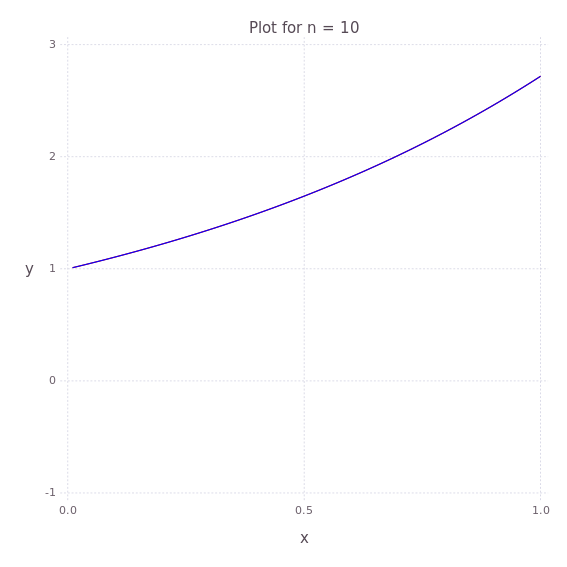
\includegraphics[width=\linewidth]{../task-5/plots/myplot-ex-10.png}\par 
    \end{multicols}
    \begin{multicols}{2}
        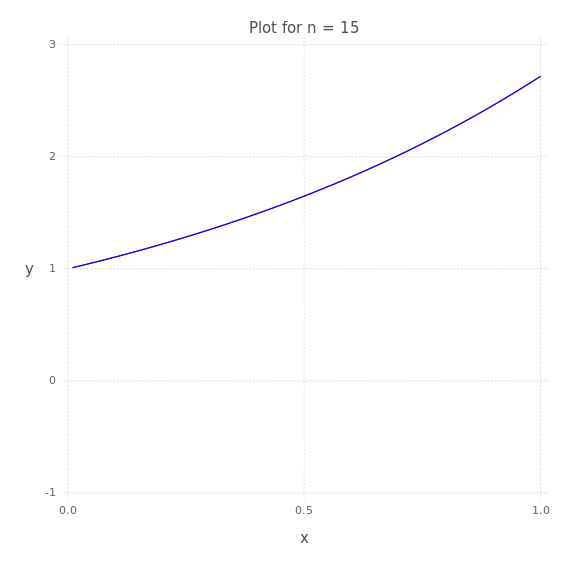
\includegraphics[width=\linewidth]{../task-5/plots/myplot-ex-15.png}\par 
    \end{multicols}
    \caption{Wykresy dla $f(x) = e^x$}    
\end{figure*}
\begin{figure*}
    \begin{multicols}{2}
        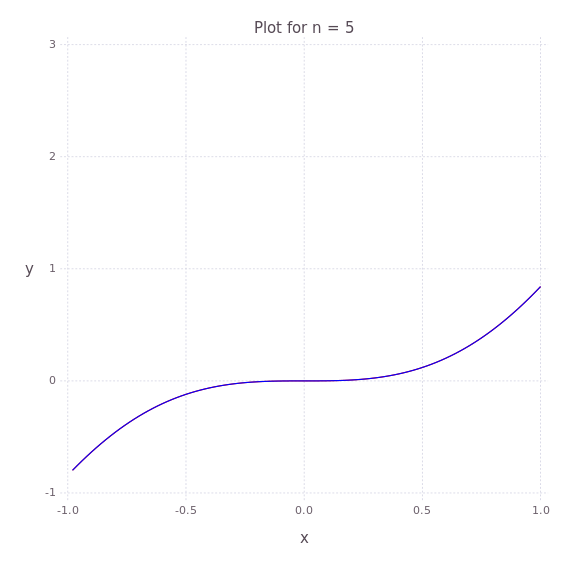
\includegraphics[width=\linewidth]{../task-5/plots/myplot-x2sinx-5.png}\par 
        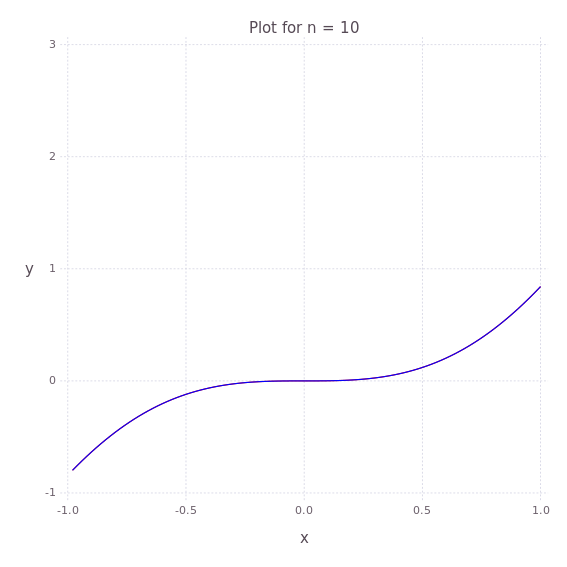
\includegraphics[width=\linewidth]{../task-5/plots/myplot-x2sinx-10.png}\par           
    \end{multicols}
    \begin{multicols}{2}
        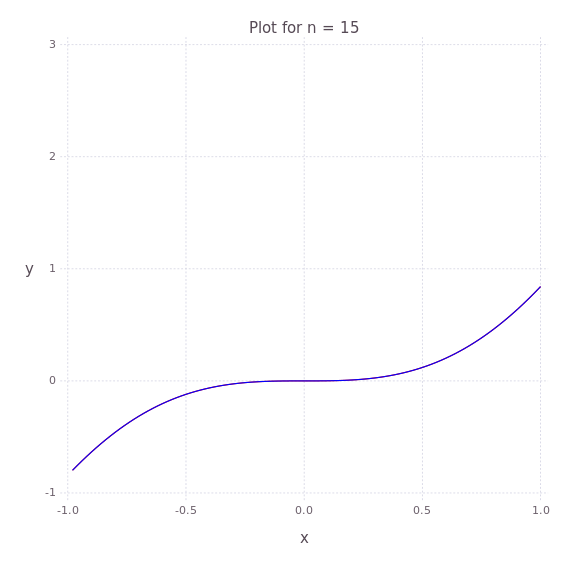
\includegraphics[width=\linewidth]{../task-5/plots/myplot-x2sinx-15.png}\par
    \end{multicols}
    \caption{Wykresy dla $g(x) = x^2 \sin(x)$}    
\end{figure*}
\subsection{Analiza wyników}
W przypadku przykładów z zadania piątego, wykresy wielomianów będących interpolacją funkcji pokryły się z wykresami tych funkcji. Interpolacja poprawnie - z pewnym małym błędem - odwzorwała zadane funkcje. Funkcje interpolowane nie spełniały żadnych warunków, które mogły powodować efekt Rungego\footnote{Efekt opisany w analizie kolejnego zadania}, mimo tego, że odległość między poszczególnymi węzłami jest stała i ich ilość nie gęstniała na krańcach przedziału.
    \newpage
    \section{Zadanie 6}
\subsection{Opis problemu}
Dla zadanego równania rekurencyjnego przeprowadź serię eksperymentów.
$$ x_{n+1} = x_{n}^2 + c\; dla\; n = 0, 1, 2,\ldots$$
Wykonać w arytmetyce $ \mathtt{Float64} $ 40 iteracji wyrażenia dla 7 zestawów danych:
\begin{enumerate}
  \item $ c = -2 \;i\; x_0 = 1 $
  \item $ c = -2 \;i\; x_0 = 2 $
  \item $ c = -2 \;i\; x_0 = 1.99999999999999 $
  \item $ c = -1 \;i\; x_0 = 1 $
  \item $ c = -1 \;i\; x_0 = -1 $
  \item $ c = -1 \;i\; x_0 = 0.75 $
  \item $ c = -1 \;i\; x_0 = 0.25 $
\end{enumerate}
\subsection{Rozwiązanie}
W celu wyliczenia zadanych rekurencji stworzyłem program w Julii, którego kod źródłowy dołączyłem do sprawozdania. Wyniki obliczeń przedstawiłem w tabeli poniżej.
\subsection{Wynik}
Spośród wszystkich zestawów danych możemy wybrać te stabilne oraz te niestabilne. \\\\
W przypadku pierwszego zestawu danych, tj. $ x_0 = 1 $ i $ c = -2 $, wyniki obliczeń pokrywają się z przewidywaniami. Każda iteracja zwraca $ -1 $. Drugi zestaw również nie przynosi zaskoczenia - każdy wynik wynosi $ -2 $. W trzecim zestawie danych operujemy na liczbie o 14 cyfrach po przecinku - jej mnożenie generuje liczbę, która nie mieści się już w arytmetyce $ \mathtt{Float64} $ i dochodzi do przybliżenia - pojawia się błąd. Każde kolejne mnożenie powoduje kolejne przybliżenie - błąd narasta. Taki algorytm z numerycznego punktu widzenia zalicza się do grupy niestabilnych i jest niepożądany. \\\\
Ciągi $ 4 $ oraz $ 5 $ tworzą cykl składający się z liczb całkowitych, w ich przypadku nigdy nie dojdzie do wyskoczenia poza precyzję arytmetyki. Te zestawy danych są stabilne.\\\\
Ostatnie dwa ciągi są o tyle interesujące, że wartość, do której - z matematycznego punktu widzenia - dążą, osiągana jest już na wysokości $ ~13 $ iteracji. Wynika to z ograniczeń precyzji arytmetyki. Liczby są na tyle małe, że arytmetyka wymaga ich zaokrąglenia. \\\\
\begin{center}
  \subsubsection*{Float64}
$$
\begin{array}{c|c|c|c|c}
algorytm & przed & \sigma & po & \sigma\\
\hline
1 & 1.0251881368e-10 & -1.1184955314e+01 & -4.2963427399e-03 & -4.2682954616e+08 \\
2 & -1.5643308870e-10 & -1.4541186645e+01 & -4.2963429987e-03 & -4.2682957187e+08 \\
3 & 0.0000000000e+00 & -1.0000000000e+00 & -4.2963428423e-03 & -4.2682955633e+08 \\
4 & 0.0000000000e+00 & -1.0000000000e+00 & -4.2963428423e-03 & -4.2682955633e+08 \\
\end{array}
$$
\subsubsection*{Float32}
$$
\begin{array}{c|c|c|c|c}
algorytm & przed & \sigma & po & \sigma\\
\hline
1 & -4.9994429946e-01 & -4.9668057661e+10 & -4.9994429946e-01 & -4.9668057661e+10 \\
2 & -4.5434570313e-01 & -4.5137965580e+10 & -4.5434570313e-01 & -4.5137965580e+10 \\
3 & -5.0000000000e-01 & -4.9673591353e+10 & -5.0000000000e-01 & -4.9673591353e+10 \\
4 & -5.0000000000e-01 & -4.9673591353e+10 & -5.0000000000e-01 & -4.9673591353e+10 \\
\end{array}
$$
  
\end{center}
\end{document}